\documentclass[tikz]{standalone}
\usepackage{fourier}
\usetikzlibrary{arrows.meta}
\usetikzlibrary{calc}
\tikzset{>=latex}
\definecolor{bookblue}{RGB}{0,173,239}
\definecolor{bookpink}{RGB}{236,0,140}
\definecolor{bookgreen}{RGB}{50,200,0}
\definecolor{bookbluearea}{RGB}{204,239,252}
\tikzstyle{blueline}=[draw=bookblue,line width=0.2mm]
\tikzstyle{pinkline}=[draw=bookpink,line width=0.2mm]
\tikzstyle{greenline}=[draw=bookgreen,line width=0.2mm]
\tikzstyle{blackline}=[draw=black,line width=0.2mm]
\tikzstyle{bluearea}=[fill=bookbluearea]

\begin{document}
  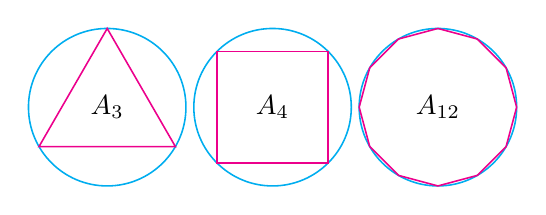
\begin{tikzpicture}
  \draw[blueline] (3.1,1) circle (1cm);
  \draw[blueline] (5.2,1) circle (1cm);
  \draw[blueline] (7.3,1) circle (1cm);
  
  \draw[pinkline] ($({3.1+cos(210)},{1+sin(210)})$) -- 
  ($({3.1+cos(330)},{1+sin(330)})$) -- 
  ($({3.1+cos( 90)},{1+sin( 90)})$) -- cycle;  %now ok
  
  \draw[pinkline] ($({5.2+cos( 45)},{1+sin( 45)})$) -- 
  ($({5.2+cos(135)},{1+sin(135)})$) -- 
  ($({5.2+cos(225)},{1+sin(225)})$) -- 
  ($({5.2+cos(315)},{1+sin(315)})$) -- cycle;  %now ok
  
  \draw[pinkline] ($({7.3+cos(  0)},{1+sin(  0)})$) -- 
  ($({7.3+cos( 30)},{1+sin( 30)})$) -- 
  ($({7.3+cos( 60)},{1+sin( 60)})$) -- 
  ($({7.3+cos( 90)},{1+sin( 90)})$) -- 
  ($({7.3+cos(120)},{1+sin(120)})$) -- 
  ($({7.3+cos(150)},{1+sin(150)})$) -- 
  ($({7.3+cos(180)},{1+sin(180)})$) -- 
  ($({7.3+cos(210)},{1+sin(210)})$) -- 
  ($({7.3+cos(240)},{1+sin(240)})$) -- 
  ($({7.3+cos(270)},{1+sin(270)})$) -- 
  ($({7.3+cos(300)},{1+sin(300)})$) -- 
  ($({7.3+cos(330)},{1+sin(330)})$) -- cycle;  %now ok
  
  \node at (3.1,1) {$A_3$};
  \node at (5.2,1) {$A_4$};
  \node at (7.3,1) {$A_{12}$};
  
  \end{tikzpicture}
\end{document}